\documentclass[10pt,a4paper]{article}

% -----------------------------------------------------------------------------
% MATHS MANTHAN | Class 10 Real Numbers Master Handbook
% Academic Year 2026--27 | Publication-quality LaTeX source with Vector TikZ.
% Compliant with latest rationalized CBSE curriculum (Euclid's Lemma deleted).
% Compile with pdfLaTeX twice for full resolution of LastPage cross-references.
% -----------------------------------------------------------------------------

\usepackage[a4paper,top=12mm,bottom=16mm,left=15mm,right=15mm,footskip=8mm]{geometry}
\usepackage[T1]{fontenc}
\usepackage{lmodern}
\usepackage{microtype}
\usepackage{amsmath,amssymb}
\usepackage[table]{xcolor}
\usepackage{array,tabularx,booktabs}
\usepackage{graphicx}
\usepackage{eso-pic}
\usepackage{tikz}
\usetikzlibrary{calc,positioning,arrows.meta,shapes.geometric,patterns}
\usepackage[most]{tcolorbox}
\usepackage{enumitem}
\usepackage{fancyhdr}
\usepackage{lastpage}
\usepackage[hidelinks]{hyperref}
\usepackage{url}

% ============================================================================
% BRAND COLOR PALETTE — MATCHED TO THE MATHS MANTHAN STANDARD
% Primary navy: #001F49 | Brand gold: #D19029
% ============================================================================
\definecolor{primary}{RGB}{0,31,73}
\definecolor{brandnavy}{RGB}{0,31,73}
\definecolor{accent}{RGB}{209,144,41}
\definecolor{brandgold}{RGB}{209,144,41}
\definecolor{secondary}{RGB}{75,85,99}
\definecolor{lightgray}{RGB}{246,248,250}
\definecolor{accentlight}{RGB}{254,250,242}
\definecolor{primarylight}{RGB}{240,244,250}

\colorlet{navy}{primary}
\colorlet{blue}{primary!82!black}
\colorlet{gold}{accent}
\colorlet{goldpale}{accentlight}
\colorlet{bluepale}{primarylight}
\colorlet{ink}{secondary}
\colorlet{muted}{secondary}
\colorlet{linegray}{primary!25}
\colorlet{reddeep}{primary}
\colorlet{redpale}{lightgray}
\colorlet{green}{primary}
\colorlet{greenpale}{primarylight}

% -----------------------------------------------------------------------------
% ROBUST LOGO DISCOVERY (TeXworks / pdfLaTeX)
% -----------------------------------------------------------------------------
\graphicspath{{./}}
\newif\ifMMLogoFound
\MMLogoFoundfalse
\def\MMLogoFile{mathsmanthan_logo.png}
\IfFileExists{mathsmanthan_logo.png}{%
  \MMLogoFoundtrue
}{%
  \IfFileExists{mathsmanthan logo.png}{%
    \def\MMLogoFile{mathsmanthan logo.png}%
    \MMLogoFoundtrue
  }{%
    \PackageWarningNoLine{MathsManthan}{Logo image not found. Put mathsmanthan_logo.png in the same folder as this .tex file}%
  }%
}

% Automatic low-opacity logo watermark on every page
\ifMMLogoFound
  \AddToShipoutPictureBG{%
    \begin{tikzpicture}[remember picture,overlay]
      \node[opacity=0.065] at (current page.center) {%
        \includegraphics[width=0.55\paperwidth,keepaspectratio]{\MMLogoFile}%
      };
    \end{tikzpicture}%
  }%
\fi

\hypersetup{
  pdftitle={Class 10 Real Numbers | Maths Manthan Handbook},
  pdfauthor={Maths Manthan Tuition Classes},
  pdfsubject={CBSE Class 10 Mathematics, Academic Year 2026--27},
  pdfkeywords={Real Numbers, Class 10, CBSE, Fundamental Theorem of Arithmetic, HCF, LCM, Irrationality, Maths Manthan}
}

\setlength{\parindent}{0pt}
\setlength{\parskip}{2.5pt}
\renewcommand{\arraystretch}{1.14}
\setlist[itemize]{leftmargin=5mm,itemsep=1.5pt,topsep=1.5pt,parsep=0pt}
\setlist[enumerate]{leftmargin=6mm,itemsep=1.5pt,topsep=1.5pt,parsep=0pt}
\setlength{\tabcolsep}{4.5pt}
\emergencystretch=2em
\hfuzz=1pt

% ============================================================================
% HEADER / FOOTER
% ============================================================================
\newcommand{\TuitionName}{{\color{primary}MATHS} {\color{accent}MANTHAN}}
\newcommand{\TuitionSub}{{\color{primary}\textbullet\ \ \text{TUITION CLASSES}\ \ \textbullet}}
\newcommand{\ContactInfo}{e-mail: contact@mathsmanthan.co.in \quad$\vert$\quad Helpline: +91-8171546558}
\newcommand{\HandbookFooterTitle}{Class 10 Real Numbers Handbook}

\pagestyle{fancy}
\fancyhf{}
\renewcommand{\headrulewidth}{0pt}
\renewcommand{\footrulewidth}{0.6pt}
\renewcommand{\footrule}{\hbox to\headwidth{\color{primary!30}\leaders\hrule height 0.6pt\hfill}}
\fancyfoot[L]{\footnotesize\href{https://mathsmanthan.co.in}{\textcolor{secondary}{\TuitionName\ $\vert$\ \HandbookFooterTitle}}}
\fancyfoot[R]{\footnotesize\textbf{\color{primary}Page \thepage\ of \pageref{LastPage}}\quad\textcolor{accent}{\textbf{Academic Year 2026--27}}}

\fancypagestyle{plain}{%
  \fancyhf{}
  \fancyfoot[L]{\footnotesize\href{https://mathsmanthan.co.in}{\textcolor{secondary}{\TuitionName\ $\vert$\ \HandbookFooterTitle}}}
  \fancyfoot[R]{\footnotesize\textbf{\color{primary}Page \thepage\ of \pageref{LastPage}}\quad\textcolor{accent}{\textbf{Academic Year 2026--27}}}
  \renewcommand{\headrulewidth}{0pt}
  \renewcommand{\footrulewidth}{0.6pt}
  \renewcommand{\footrule}{\hbox to\headwidth{\color{primary!30}\leaders\hrule height 0.6pt\hfill}}
}

% Reusable design components
\newcommand{\BrandMark}{%
  \ifMMLogoFound
    \includegraphics[width=22mm,height=22mm,keepaspectratio]{\MMLogoFile}%
  \else
    
\begin{tikzpicture}[baseline=-0.6ex]
      \fill[navy,rounded corners=2.2pt] (0,0) rectangle (1.45,1.05);
      \draw[gold,line width=1.2pt] (0.15,0.15)--(1.30,0.15);
      \node[text=white,font=\sffamily\bfseries\Large] at (0.725,0.59) {MM};
    \end{tikzpicture}%
  \fi
}

\newcommand{\chapterbanner}[4]{%
  \begin{tcolorbox}[enhanced,colback=bluepale,colframe=bluepale,boxrule=0pt,arc=2mm,
    left=4mm,right=4mm,top=2mm,bottom=2mm]
    {\footnotesize\bfseries\color{gold}CHAPTER #1\hfill\color{blue}#4}\par\vspace{0.6mm}
    {\LARGE\bfseries\color{navy}#2}\par
    {\small\color{muted}#3}
  \end{tcolorbox}\vspace{1mm}
}

\newcommand{\subhead}[1]{%
  \vspace{1mm}{\large\bfseries\color{navy}#1}\par\vspace{0.4mm}
  {\color{gold}\rule{13mm}{1.2pt}}\par\vspace{0.8mm}
}

\newtcolorbox{formulaBox}[1][]{enhanced,breakable,colback=goldpale,colframe=gold!65!black,
  boxrule=0.5pt,arc=1.5mm,left=3mm,right=3mm,top=1.8mm,bottom=1.8mm,
  before skip=2.5pt,after skip=3.5pt,#1}
\newtcolorbox{conceptBox}[1][]{enhanced,breakable,colback=bluepale,colframe=blue!25,
  boxrule=0.4pt,arc=1.5mm,left=3mm,right=3mm,top=1.8mm,bottom=1.8mm,
  before skip=2.5pt,after skip=3.5pt,#1}
\newtcolorbox{warningBox}[1][]{enhanced,breakable,colback=redpale,colframe=reddeep!45,
  boxrule=0.45pt,arc=1.5mm,left=3mm,right=3mm,top=1.8mm,bottom=1.8mm,
  before skip=2.5pt,after skip=3.5pt,#1}
\newtcolorbox{successBox}[1][]{enhanced,breakable,colback=greenpale,colframe=green!35,
  boxrule=0.45pt,arc=1.5mm,left=3mm,right=3mm,top=1.8mm,bottom=1.8mm,
  before skip=2.5pt,after skip=3.5pt,#1}

\newcommand{\CoreTag}{\tcbox[colback=greenpale,colframe=green!40,boxrule=.3pt,arc=1mm,left=1.5mm,right=1.5mm,top=.5mm,bottom=.5mm]{\scriptsize\bfseries\color{green}CORE SYLLABUS}}
\newcommand{\ExamTag}{\tcbox[colback=bluepale,colframe=blue!25,boxrule=.3pt,arc=1mm,left=1.5mm,right=1.5mm,top=.5mm,bottom=.5mm]{\scriptsize\bfseries\color{blue}EXAM STRATEGY}}
\newcommand{\TrapTag}{\tcbox[colback=redpale,colframe=reddeep!40,boxrule=.3pt,arc=1mm,left=1.5mm,right=1.5mm,top=.5mm,bottom=.5mm]{\scriptsize\bfseries\color{reddeep}TRAP ALERT}}
\newcommand{\WorkedTag}{\tcbox[colback=bluepale,colframe=blue!25,boxrule=.3pt,arc=1mm,left=1.5mm,right=1.5mm,top=.5mm,bottom=.5mm]{\scriptsize\bfseries\color{blue}WORKED MODEL}}
\newcommand{\SupportTag}{\tcbox[colback=accentlight,colframe=gold!55!black,boxrule=.3pt,arc=1mm,left=1.5mm,right=1.5mm,top=.5mm,bottom=.5mm]{\scriptsize\bfseries\color{primary}SUPPORTING SKILL}}
\newcommand{\ReferenceTag}{\tcbox[colback=bluepale,colframe=blue!25,boxrule=.3pt,arc=1mm,left=1.5mm,right=1.5mm,top=.5mm,bottom=.5mm]{\scriptsize\bfseries\color{primary}REFERENCE MATRIX}}

\begin{document}

% =============================================================================
% PAGE 1: COVER PAGE
% =============================================================================
\thispagestyle{fancy}
\vspace*{0mm}

\noindent
\makebox[0pt][l]{%
  \raisebox{-0.80cm}[0pt][0pt]{%
    \href{https://mathsmanthan.co.in}{%
      \BrandMark%
    }%
  }%
}%
\parbox{\textwidth}{%
  \centering
  \href{https://mathsmanthan.co.in}{%
    {\fontsize{23pt}{23pt}\selectfont\bfseries \TuitionName}\\[3pt]
    {\footnotesize\bfseries \TuitionSub}%
  }\\[2pt]
  {\scriptsize\color{secondary} \ContactInfo}
}

\vspace{5pt}
\noindent{\color{primary}\rule{0.72\textwidth}{1.5pt}}\hfill{\color{accent}\rule{0.26\textwidth}{1.5pt}}

\vspace{3mm}
\begin{center}
  {\large\bfseries\color{muted}CBSE CLASS 10 \;|\; MATHEMATICS}\\[3mm]
  {\fontsize{26}{30}\selectfont\bfseries\color{navy}REAL NUMBERS}\\[2.5mm]
  {\Large\color{blue}Fundamental Theorem of Arithmetic, Divisibility \& Irrationality Proofs}\\[2.5mm]
  {\large\color{gold}\bfseries Academic Year 2026--27}
\end{center}

\vspace{2mm}
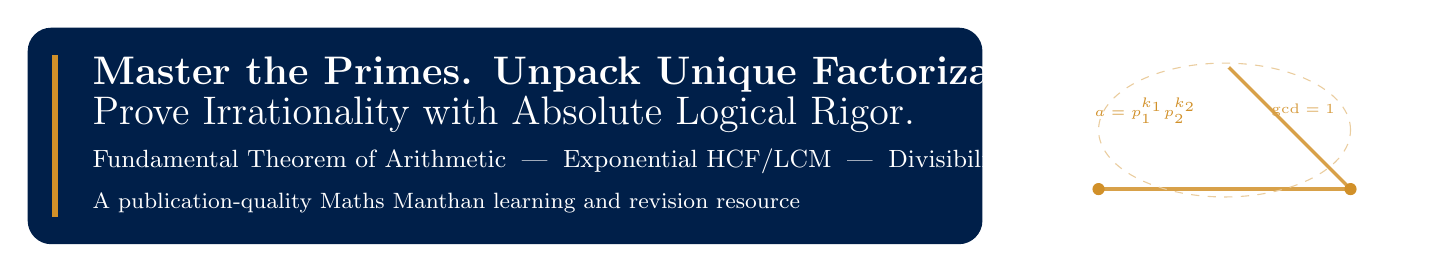
\begin{tikzpicture}
  \fill[navy,rounded corners=3mm] (0,0) rectangle (\textwidth,2.75);
  \draw[gold,line width=2pt] (0.35,0.35)--(0.35,2.40);
  \node[anchor=west,text=white,font=\bfseries\Large] at (0.7,2.15) {Master the Primes. Unpack Unique Factorization.};
  \node[anchor=west,text=white,font=\Large] at (0.7,1.65) {Prove Irrationality with Absolute Logical Rigor.};
  \node[anchor=west,text=white,font=\small] at (0.7,1.05) {Fundamental Theorem of Arithmetic \;|\; Exponential HCF/LCM \;|\; Divisibility Lemma \;|\; Contradiction Proofs};
  \node[anchor=west,text=white!75,font=\footnotesize] at (0.7,0.52) {A publication-quality Maths Manthan learning and revision resource};
  
  % Decorative Real Numbers Mathematical Graphic in gold & white
  \draw[gold!85, line width=1.5pt] (13.6, 0.70) -- (16.8, 0.70);
  \draw[white, line width=1.2pt] (13.6, 0.70) -- (15.2, 2.30);
  \draw[gold!85, line width=1.2pt] (15.2, 2.30) -- (16.8, 0.70);
  \fill[gold] (13.6, 0.70) circle (2.2pt);
  \fill[white] (15.2, 2.30) circle (2.2pt);
  \fill[gold] (16.8, 0.70) circle (2.2pt);
  \node[text=white, font=\bfseries\footnotesize] at (15.2, 1.25) {$\sqrt{p} \notin \mathbb{Q}$};
  \node[text=gold, font=\bfseries\tiny] at (14.2, 1.70) {$a = p_1^{k_1}p_2^{k_2}$};
  \node[text=gold!90, font=\bfseries\tiny] at (16.2, 1.70) {$\gcd=1$};
  \draw[gold!45, dashed] (15.2, 1.45) circle (1.6cm and 0.85cm);
\end{tikzpicture}

\vspace{2.5mm}
\begin{minipage}[t]{0.485\textwidth}
  \begin{conceptBox}[title=What this handbook includes,fonttitle=\bfseries\color{navy}]
    \begin{itemize}
      \item Set-theoretic foundations of $\mathbb{R}$: $\mathbb{N} \subset \mathbb{W} \subset \mathbb{Z} \subset \mathbb{Q} \subset \mathbb{R}$ and the Real Line continuum.
      \item The Fundamental Theorem of Arithmetic (FTA) and Canonical Prime Decomposition ($n = \prod p_i^{a_i}$).
      \item The Exponential Power Law of HCF ($\min$) and LCM ($\max$).
      \item The Dual-Number Product Theorem $\text{HCF} \times \text{LCM} = a \times b$ and why it strictly fails for three numbers.
      \item Real-world word problems decision framework (HCF vs LCM).
      \item Complete formal proofs for irrationality of $\sqrt{2}, \sqrt{3}, \sqrt{5}$ and linear combinations ($a \pm b\sqrt{c}$).
    \end{itemize}
  \end{conceptBox}
\end{minipage}\hfill
\begin{minipage}[t]{0.485\textwidth}
  \begin{formulaBox}[title=How to use it for maximum marks,fonttitle=\bfseries\color{navy}]
    \raggedright In irrationality proofs, always explicitly state that $a$ and $b$ are \textbf{coprime integers with $b \ne 0$} ($\gcd(a, b) = 1$) to avoid a mandatory 1-mark deduction. In word problems, state the prime factorizations in exponential index notation before applying $\min$ or $\max$ powers. Never write $\text{HCF}(a, b, c) \times \text{LCM}(a, b, c) = a \cdot b \cdot c$ for 3 numbers.
  \end{formulaBox}
\end{minipage}

\vspace{1.5mm}
\begin{warningBox}[title=Official syllabus scope (CBSE Class X 2026--27),fonttitle=\bfseries\color{navy}]
  The published CBSE Class X curriculum for 2026--27 prescribes \textbf{Fundamental Theorem of Arithmetic -- statements after reviewing work done earlier and after illustrating and motivating through examples, Proofs of irrationality of $\sqrt{2}, \sqrt{3}, \sqrt{5}$.} \\
  \textbf{Strictly Excluded Topics (Deleted from Rationalized Syllabus):} \\
  Section 1.2: Euclid's Division Lemma ($a = bq + r$) and its algorithmic application to find HCF are \textbf{completely deleted}. Questions representing integers as $6q+1$, $6q+3$ or proving squares of forms $(3m)^2$ are excluded. Section 1.4: Revisiting Rational Numbers and Their Decimal Expansions (terminating criteria $q = 2^n 5^m$) is \textbf{completely deleted}.\par
  {\scriptsize Source: \href{https://cbseacademic.nic.in/web_material/CurriculumMain27/SecPart1/Maths_SecP1X_2026-27.pdf}{CBSE Mathematics Class X Curriculum (2026--27), Unit I: Number Systems, Chapter 1}.}
\end{warningBox}

\vfill
\begin{center}
  {\small\bfseries\color{navy}Maths Manthan Tuition Classes}\\
  {\footnotesize\color{muted}contact@mathsmanthan.co.in \quad\textbar\quad +91-8171546558}\\
  {\footnotesize\url{https://mathsmanthan.co.in}}\\[2mm]
  {\scriptsize\color{muted}Prepared for learning and revision \;--\; not an official CBSE publication.}
\end{center}

\newpage

% =============================================================================
% PAGE 2: GEOMETRIC & SET-THEORETIC FOUNDATIONS OF REAL NUMBERS
% =============================================================================
\thispagestyle{fancy}
\vspace*{0mm}

\chapterbanner{1}{GEOMETRIC \& SET FOUNDATIONS}{The Number Hierarchy, Real Line Continuum \& Decimal Duality}{\CoreTag}

\subhead{Module 1 $\vert$ The Set-Theoretic Hierarchy of Numbers}

The system of Real Numbers ($\mathbb{R}$) is built hierarchically through successive algebraic extensions:

\begin{center}
{\small
\begin{tabularx}{\textwidth}{@{}lllX@{}}
  \toprule
  \textbf{\color{navy}Set Name} & \textbf{\color{navy}Symbol} & \textbf{\color{navy}Formal Mathematical Definition} & \textbf{\color{navy}Structural Role \& Intuition} \\
  \midrule
  \textbf{Natural Numbers} & $\mathbb{N}$ & $\{1, 2, 3, 4, 5, \dots\}$ & Primitive discrete counting elements. \\
  \addlinespace[1.5pt]
  \textbf{Whole Numbers} & $\mathbb{W}$ & $\{0\} \cup \mathbb{N} = \{0, 1, 2, 3, \dots\}$ & Introduces the additive identity (null quantity). \\
  \addlinespace[1.5pt]
  \textbf{Integers} & $\mathbb{Z}$ & $\{\dots, -2, -1, 0, 1, 2, \dots\}$ & Introduces additive inverses (negative quantities). \\
  \addlinespace[1.5pt]
  \textbf{Rational Numbers} & $\mathbb{Q}$ & $\left\{ \dfrac{p}{q} \;\middle|\; p, q \in \mathbb{Z}, \, q \ne 0, \, \gcd(p, q) = 1 \right\}$ & Closed under division; expresses all fractional ratios. \\
  \addlinespace[1.5pt]
  \textbf{Irrational Numbers} & $\mathbb{Q}'$ / $\mathbb{I}$ & $\{ x \in \mathbb{R} \mid x \notin \mathbb{Q} \}$ & Numbers that cannot be written as a fraction of integers. \\
  \addlinespace[1.5pt]
  \textbf{Real Numbers} & $\mathbb{R}$ & $\mathbb{Q} \cup \mathbb{Q}'$ & Complete, gapless continuous geometric number line. \\
  \bottomrule
\end{tabularx}}
\end{center}

\vspace{0.5mm}
\begin{minipage}[t]{0.54\textwidth}
  \subhead{Module 2 $\vert$ Decimal Representation Duality}
  \begin{conceptBox}[title=Decimal Characterization of Real Numbers,fonttitle=\bfseries\color{navy}]
    Every real number possesses a unique decimal expansion:
    \begin{itemize}
      \item \textbf{Rational ($\mathbb{Q}$):} Decimal expansion is either:
        \begin{enumerate}[label=(\alph*),leftmargin=5mm,itemsep=0pt]
          \item \textbf{Terminating:} e.g., $\frac{3}{8} = 0.375$.
          \item \textbf{Non-terminating Recurring (Periodic):} e.g., $\frac{1}{3} = 0.333\dots = 0.\overline{3}$, $\frac{1}{7} = 0.\overline{142857}$.
        \end{enumerate}
      \item \textbf{Irrational ($\mathbb{Q}'$):} Decimal expansion is \textbf{strictly non-terminating and non-recurring}.
        \begin{itemize}[leftmargin=4mm,itemsep=0pt]
          \item $\sqrt{2} = 1.41421356237\dots$ (No repeating block).
          \item $\pi = 3.14159265358\dots$ (Cannot be matched by any ratio).
        \end{itemize}
    \end{itemize}
  \end{conceptBox}
\end{minipage}\hfill
\begin{minipage}[t]{0.43\textwidth}
  \begin{center}
  \vspace{2mm}
  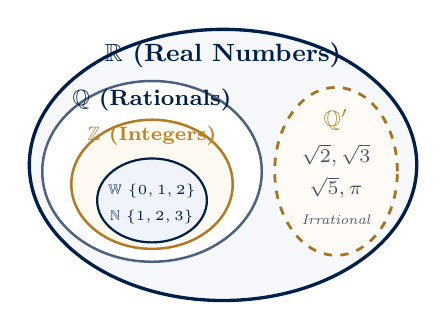
\begin{tikzpicture}[scale=0.82]
    % Nested Sets
    \draw[navy, line width=1.2pt, fill=bluepale!60] (0,0) ellipse (3.0cm and 2.1cm);
    \node[navy, font=\bfseries\small] at (0, 1.7) {$\mathbb{R}$ (Real Numbers)};

    % Rationals vs Irrationals split
    \draw[navy!70, line width=0.9pt, fill=white] (-1.1,-0.1) ellipse (1.7cm and 1.4cm);
    \node[navy, font=\bfseries\footnotesize] at (-1.1, 1.0) {$\mathbb{Q}$ (Rationals)};

    % Integers
    \draw[gold!85!black, line width=0.9pt, fill=goldpale] (-1.1,-0.3) ellipse (1.25cm and 1.0cm);
    \node[gold!90!black, font=\bfseries\scriptsize] at (-1.1, 0.45) {$\mathbb{Z}$ (Integers)};

    % Whole & Naturals
    \draw[primary, line width=0.8pt, fill=bluepale] (-1.1,-0.55) ellipse (0.85cm and 0.65cm);
    \node[primary, font=\bfseries\tiny] at (-1.1, -0.4) {$\mathbb{W} \; \{0, 1, 2\}$};
    \node[primary, font=\bfseries\tiny] at (-1.1, -0.8) {$\mathbb{N} \; \{1, 2, 3\}$};

    % Irrationals block
    \draw[accent!80!black, line width=1pt, dashed, fill=goldpale!50] (1.75,-0.1) ellipse (0.95cm and 1.3cm);
    \node[accent!90!black, font=\bfseries\footnotesize] at (1.75, 0.7) {$\mathbb{Q}'$};
    \node[secondary, font=\scriptsize] at (1.75, 0.15) {$\sqrt{2}, \sqrt{3}$};
    \node[secondary, font=\scriptsize] at (1.75, -0.35) {$\sqrt{5}, \pi$};
    \node[secondary, font=\tiny\itshape] at (1.75, -0.85) {Irrational};
  \end{tikzpicture}
  \end{center}
\end{minipage}

\vspace{1mm}
\subhead{Module 3 $\vert$ The Real Number Line Continuum (Dedekind--Cantor Completeness)}

\begin{formulaBox}[title=The Fundamental Geometric Continuum Axiom,fonttitle=\bfseries\color{navy}]
  \textbf{The Dedekind--Cantor Axiom:} To every real number there corresponds a \textbf{unique point} on the number line, and conversely, to every point on the number line there corresponds \textbf{exactly one real number}. The rationals $\mathbb{Q}$ are dense but full of holes; the irrationals $\mathbb{Q}'$ fill every single geometric gap.
\end{formulaBox}

\begin{center}
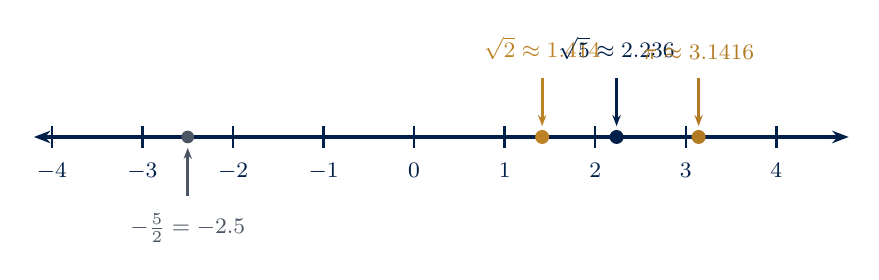
\begin{tikzpicture}[scale=1.15]
  % Number line axis
  \draw[navy, line width=1.2pt, {Stealth[length=6pt]}-{Stealth[length=6pt]}] (-4.2,0) -- (4.8,0);
  
  % Integer ticks
  \foreach \x in {-4,-3,-2,-1,0,1,2,3,4} {
    \draw[navy, line width=0.9pt] (\x, 0.12) -- (\x, -0.12);
    \node[below=2pt, navy, font=\bfseries\footnotesize] at (\x, -0.12) {$\x$};
  }

  % Plotted irrational points
  % sqrt(2) approx 1.414
  \draw[gold!90!black, line width=1.1pt, -{Stealth[length=4pt]}] (1.414, 0.65) -- (1.414, 0.12);
  \fill[gold!90!black] (1.414, 0) circle (2.2pt);
  \node[above=3pt, gold!90!black, font=\bfseries\footnotesize] at (1.414, 0.65) {$\sqrt{2} \approx 1.414$};

  % sqrt(5) approx 2.236
  \draw[primary, line width=1.1pt, -{Stealth[length=4pt]}] (2.236, 0.65) -- (2.236, 0.12);
  \fill[primary] (2.236, 0) circle (2.2pt);
  \node[above=3pt, primary, font=\bfseries\footnotesize] at (2.236, 0.65) {$\sqrt{5} \approx 2.236$};

  % pi approx 3.14159
  \draw[gold!85!black, line width=1.1pt, -{Stealth[length=4pt]}] (3.14159, 0.65) -- (3.14159, 0.12);
  \fill[gold!85!black] (3.14159, 0) circle (2.2pt);
  \node[above=3pt, gold!85!black, font=\bfseries\footnotesize] at (3.14159, 0.65) {$\pi \approx 3.1416$};

  % negative rational -5/2 = -2.5
  \draw[secondary, line width=1pt, -{Stealth[length=4pt]}] (-2.5, -0.65) -- (-2.5, -0.12);
  \fill[secondary] (-2.5, 0) circle (2pt);
  \node[below=3pt, secondary, font=\bfseries\footnotesize] at (-2.5, -0.65) {$-\frac{5}{2} = -2.5$};
\end{tikzpicture}
\end{center}

\newpage

% =============================================================================
% PAGE 3: THE FUNDAMENTAL THEOREM OF ARITHMETIC (FTA)
% =============================================================================
\thispagestyle{fancy}
\vspace*{0mm}

\chapterbanner{1}{FUNDAMENTAL THEOREM OF ARITHMETIC}{Prime Building Blocks, Uniqueness \& Canonical Representation}{\CoreTag}

\subhead{Module 1 $\vert$ The Fundamental Theorem of Arithmetic (FTA)}

\begin{conceptBox}[title={Formal Statement of the Theorem (Carl Friedrich Gauss, 1801)},fonttitle=\bfseries\color{navy}]
  \textbf{Theorem:} \textit{Every composite number can be expressed (factorized) as a product of primes, and this factorization is \textbf{unique}, apart from the order in which the prime factors occur.}
  \begin{itemize}
    \item \textbf{Existence Clause:} Any integer $n > 1$ can be broken down into a product of prime building blocks.
    \item \textbf{Uniqueness Clause:} There is only \textbf{one singular set of prime powers} that produces $n$. No matter which method or branching sequence is used, the final prime components are identical!
  \end{itemize}
\end{conceptBox}

\vspace{0.5mm}
\subhead{Module 2 $\vert$ Canonical Prime Decomposition}

Writing primes in ascending order gives the \textbf{Canonical Representation} of an integer $n$:
$$\mathbf{n = p_1^{a_1} \cdot p_2^{a_2} \cdot p_3^{a_3} \cdots p_k^{a_k} = \prod_{i=1}^k p_i^{a_i}}$$
where $p_1 < p_2 < p_3 < \dots < p_k$ are distinct positive primes and $a_i \in \mathbb{N}$ are their respective natural multiplicities.

\vspace{0.5mm}
\begin{minipage}[t]{0.54\textwidth}
  \subhead{Module 3 $\vert$ The Factor Tree Algorithm}
  A \textbf{Factor Tree} is a visual recursive algorithm for obtaining canonical prime decomposition:
  \begin{enumerate}[leftmargin=5mm,itemsep=1.5pt]
    \item Write the composite number $n$ at the root.
    \item Branch $n$ into its smallest prime divisor $p$ and quotient $q$.
    \item Circle the prime factor $p$ (leaf node: terminated branch).
    \item If quotient $q$ is composite, repeat the branching process.
    \item Termination occurs when all leaf nodes are prime numbers.
    \item Collect identical prime leaves into exponential powers.
  \end{enumerate}
\end{minipage}\hfill
\begin{minipage}[t]{0.43\textwidth}
  \begin{center}
  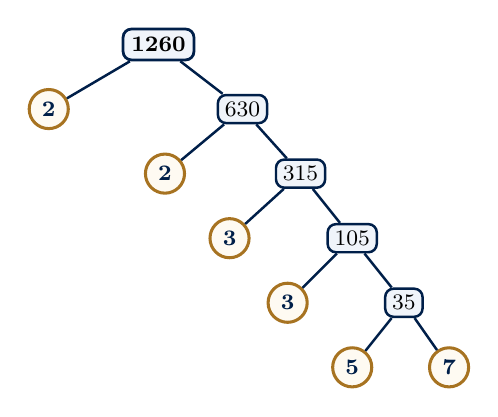
\begin{tikzpicture}[scale=0.82, every node/.style={font=\footnotesize}]
    % Root: 1260
    \node[draw=navy, fill=bluepale, rounded corners=3pt, line width=1pt, inner sep=3pt] (N) at (2.5, 4.4) {\textbf{1260}};

    % Level 1: 2 and 630
    \node[draw=gold!80!black, fill=goldpale, circle, line width=1.1pt, inner sep=2.5pt] (P1) at (0.8, 3.4) {\textbf{\color{navy}2}};
    \node[draw=navy, fill=bluepale, rounded corners=3pt, line width=0.9pt, inner sep=2.5pt] (Q1) at (3.8, 3.4) {630};
    \draw[navy, line width=0.9pt] (N) -- (P1);
    \draw[navy, line width=0.9pt] (N) -- (Q1);

    % Level 2: 2 and 315
    \node[draw=gold!80!black, fill=goldpale, circle, line width=1.1pt, inner sep=2.5pt] (P2) at (2.6, 2.4) {\textbf{\color{navy}2}};
    \node[draw=navy, fill=bluepale, rounded corners=3pt, line width=0.9pt, inner sep=2.5pt] (Q2) at (4.7, 2.4) {315};
    \draw[navy, line width=0.9pt] (Q1) -- (P2);
    \draw[navy, line width=0.9pt] (Q1) -- (Q2);

    % Level 3: 3 and 105
    \node[draw=gold!80!black, fill=goldpale, circle, line width=1.1pt, inner sep=2.5pt] (P3) at (3.6, 1.4) {\textbf{\color{navy}3}};
    \node[draw=navy, fill=bluepale, rounded corners=3pt, line width=0.9pt, inner sep=2.5pt] (Q3) at (5.5, 1.4) {105};
    \draw[navy, line width=0.9pt] (Q2) -- (P3);
    \draw[navy, line width=0.9pt] (Q2) -- (Q3);

    % Level 4: 3 and 35
    \node[draw=gold!80!black, fill=goldpale, circle, line width=1.1pt, inner sep=2.5pt] (P4) at (4.5, 0.4) {\textbf{\color{navy}3}};
    \node[draw=navy, fill=bluepale, rounded corners=3pt, line width=0.9pt, inner sep=2.5pt] (Q4) at (6.3, 0.4) {35};
    \draw[navy, line width=0.9pt] (Q3) -- (P4);
    \draw[navy, line width=0.9pt] (Q3) -- (Q4);

    % Level 5: 5 and 7
    \node[draw=gold!80!black, fill=goldpale, circle, line width=1.1pt, inner sep=2.5pt] (P5) at (5.5, -0.6) {\textbf{\color{navy}5}};
    \node[draw=gold!80!black, fill=goldpale, circle, line width=1.1pt, inner sep=2.5pt] (P6) at (7.0, -0.6) {\textbf{\color{navy}7}};
    \draw[navy, line width=0.9pt] (Q4) -- (P5);
    \draw[navy, line width=0.9pt] (Q4) -- (P6);
  \end{tikzpicture}
  \par\vspace{0.5mm}
  {\footnotesize\bfseries\color{navy}$1260 = 2^2 \times 3^2 \times 5 \times 7$}
  \end{center}
\end{minipage}

\vspace{1mm}
\begin{formulaBox}[title=Worked Model: Finding Unknown Missing Branches in a Factor Tree,fonttitle=\bfseries\color{navy}]
  \textbf{Board Problem:} In a given factor tree, a parent node $x$ splits into $3$ and $y$, and $y$ splits into $5$ and $13$. Determine the values of $x$ and $y$. \\
  \textbf{Solution by Inversion:}\par
  \textbf{Step 1: Compute child node $y$:} $y = 5 \times 13 = \mathbf{65}$. \\
  \textbf{Step 2: Compute parent node $x$:} $x = 3 \times y = 3 \times 65 = \mathbf{195}$. \\
  \textbf{Verification:} Canonical prime factorization of $195 = 3 \times 5 \times 13$. Uniqueness guarantees singular solution.
\end{formulaBox}

\newpage

% =============================================================================
% PAGE 4: THE EXPONENTIAL LAW OF HCF AND LCM
% =============================================================================
\thispagestyle{fancy}
\vspace*{0mm}

\chapterbanner{1}{THE EXPONENTIAL LAW OF HCF \& LCM}{Min/Max Power Protocols \& The Two-Number Product Theorem}{\CoreTag}

\subhead{Module 1 $\vert$ Exponential Definitions of HCF and LCM}

Let the canonical prime factorizations of two natural numbers $a$ and $b$ be expressed across all involved primes:
$$a = p_1^{\alpha_1} p_2^{\alpha_2} \cdots p_k^{\alpha_k} \qquad \text{and} \qquad b = p_1^{\beta_1} p_2^{\beta_2} \cdots p_k^{\beta_k} \quad (\alpha_i, \beta_i \ge 0)$$

\begin{formulaBox}[title=The Fundamental Power Laws for HCF and LCM,fonttitle=\bfseries\color{navy}]
  \begin{itemize}[leftmargin=4mm]
    \item \textbf{Highest Common Factor (HCF):} Product of the \textbf{smallest powers} of each common prime factor:
      $$\mathbf{\text{HCF}(a, b) = \prod_{i=1}^k p_i^{\min(\alpha_i, \beta_i)} = p_1^{\min(\alpha_1, \beta_1)} \cdot p_2^{\min(\alpha_2, \beta_2)} \cdots p_k^{\min(\alpha_k, \beta_k)}}$$
    \item \textbf{Lowest Common Multiple (LCM):} Product of the \textbf{greatest powers} of each prime factor involved:
      $$\mathbf{\text{LCM}(a, b) = \prod_{i=1}^k p_i^{\max(\alpha_i, \beta_i)} = p_1^{\max(\alpha_1, \beta_1)} \cdot p_2^{\max(\alpha_2, \beta_2)} \cdots p_k^{\max(\alpha_k, \beta_k)}}$$
  \end{itemize}
\end{formulaBox}

\vspace{0.5mm}
\subhead{Module 2 $\vert$ The Dual-Number Product Theorem}

\begin{minipage}[t]{0.56\textwidth}
  \begin{conceptBox}[title=Theorem: Product Law for Two Numbers,fonttitle=\bfseries\color{navy}]
    For any two positive integers $a$ and $b$:
    $$\mathbf{\text{HCF}(a, b) \times \text{LCM}(a, b) = a \times b}$$
    \textbf{Mathematical Proof via Exponents:} \\
    For every prime factor $p_i$, the sum of exponents is:
    $$\min(\alpha_i, \beta_i) + \max(\alpha_i, \beta_i) = \alpha_i + \beta_i$$
    Taking the product across all primes:
    $$\prod p_i^{\min(\alpha_i, \beta_i)} \times \prod p_i^{\max(\alpha_i, \beta_i)} = \prod p_i^{\alpha_i + \beta_i} = a \times b$$
    $$\therefore \mathbf{\text{LCM}(a, b) = \frac{a \times b}{\text{HCF}(a, b)}}, \qquad \mathbf{\text{HCF}(a, b) = \frac{a \times b}{\text{LCM}(a, b)}}$$
  \end{conceptBox}
\end{minipage}\hfill
\begin{minipage}[t]{0.42\textwidth}
  \begin{center}
  \vspace{1mm}
  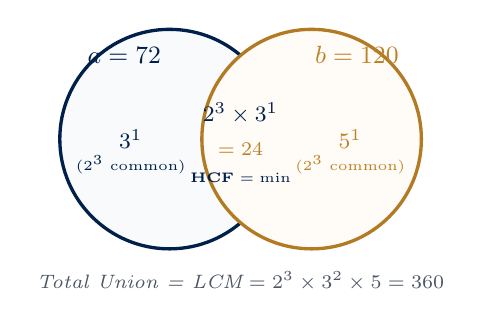
\begin{tikzpicture}[scale=0.82]
    % Venn diagram for a=72, b=120
    \draw[navy, line width=1.2pt, fill=bluepale!50] (-1.1,0) circle (1.7cm);
    \draw[gold!85!black, line width=1.2pt, fill=goldpale!50] (1.1,0) circle (1.7cm);

    % Labels
    \node[navy, font=\bfseries\small] at (-1.8, 1.3) {$a = 72$};
    \node[gold!90!black, font=\bfseries\small] at (1.8, 1.3) {$b = 120$};

    % Exclusive a factors
    \node[navy, font=\footnotesize] at (-1.7, 0) {$3^1$};
    \node[navy, font=\tiny\color{secondary}] at (-1.7, -0.4) {$(2^3 \text{ common})$};

    % Intersection: HCF
    \node[navy, font=\bfseries\footnotesize] at (0, 0.4) {$2^3 \times 3^1$};
    \node[gold!90!black, font=\bfseries\scriptsize] at (0, -0.15) {$= 24$};
    \node[primary, font=\bfseries\tiny] at (0, -0.6) {$\mathbf{HCF = \min}$};

    % Exclusive b factors
    \node[gold!90!black, font=\footnotesize] at (1.7, 0) {$5^1$};
    \node[gold!90!black, font=\tiny\color{secondary}] at (1.7, -0.4) {$(2^3 \text{ common})$};

    % Union note
    \node[below, secondary, font=\scriptsize\itshape] at (0, -1.9) {Total Union = $\text{LCM} = 2^3 \times 3^2 \times 5 = 360$};
  \end{tikzpicture}
  \end{center}
\end{minipage}

\vspace{0.8mm}
\subhead{Module 3 $\vert$ The Three-Number Fallacy (CBSE Lethal Trap)}

\begin{warningBox}[title=Critical Warning: Product Law Fails for Three Numbers!,fonttitle=\bfseries\color{navy}]
  \textbf{CBSE Board Trap:} It is \textbf{STRICTLY FALSE} that $\text{HCF}(a, b, c) \times \text{LCM}(a, b, c) = a \times b \times c$! \\
  \textbf{Concrete Counterexample:} Let $a = 6 = 2 \times 3$, $b = 8 = 2^3$, $c = 12 = 2^2 \times 3$.
  \begin{itemize}[itemsep=0pt]
    \item $\text{HCF}(6, 8, 12) = 2^1 = \mathbf{2}$; \quad $\text{LCM}(6, 8, 12) = 2^3 \times 3 = \mathbf{24}$.
    \item $\text{LHS} = \text{HCF} \times \text{LCM} = 2 \times 24 = \mathbf{48}$.
    \item $\text{RHS} = a \times b \times c = 6 \times 8 \times 12 = \mathbf{576}$. \quad \textbf{Clearly, $48 \ne 576$!}
  \end{itemize}
  \textbf{True Formula for 3 Numbers (For Reference):}
  $$\text{LCM}(a, b, c) = \frac{a \cdot b \cdot c \cdot \text{HCF}(a, b, c)}{\text{HCF}(a, b) \cdot \text{HCF}(b, c) \cdot \text{HCF}(c, a)}$$
\end{warningBox}

\newpage

% =============================================================================
% PAGE 5: WORD PROBLEMS & REAL-WORLD DECISION ENGINE
% =============================================================================
\thispagestyle{fancy}
\vspace*{0mm}

\chapterbanner{1}{WORD PROBLEMS DECISION ENGINE}{Semantic Triggers, Recurrence Cycles \& Optimal Grouping}{\WorkedTag}

\subhead{Module 1 $\vert$ The Semantic Trigger Decision Framework}

When confronted with real-world situational word problems, identify the governing mathematical structure:

\begin{center}
{\footnotesize
\begin{tabularx}{\textwidth}{@{}lXX@{}}
  \toprule
  \textbf{\color{navy}Diagnostic Criteria} & \textbf{\color{navy}HCF Model (Subdivision / Partition)} & \textbf{\color{navy}LCM Model (Multiple / Recurrence)} \\
  \midrule
  \textbf{Physical Objective} & Dividing larger quantities into smaller, equal groups with \textbf{no remainder}. & Finding a common cycle, synchronization point, or smallest expanded quantity. \\
  \addlinespace[1.5pt]
  \textbf{Semantic Keywords} & \textbf{Maximum}, largest, greatest, highest capacity, longest tape, equal heaps, minimum number of stacks. & \textbf{Minimum}, least, smallest, bells chiming together, traffic lights changing, runners circling a track. \\
  \addlinespace[1.5pt]
  \textbf{Size Constraint} & The result is \textbf{smaller than or equal to} given values: $\text{HCF} \le \min(a, b)$. & The result is \textbf{larger than or equal to} given values: $\text{LCM} \ge \max(a, b)$. \\
  \bottomrule
\end{tabularx}}
\end{center}

\vspace{-1mm}
\subhead{Module 2 $\vert$ Worked Board Archetype 1: Circular Sports Track (LCM Model)}
\vspace{-1mm}

\begin{minipage}[t]{0.58\textwidth}
  \textbf{Problem:} Sonia takes 18 min and Ravi takes 12 min for one round of a sports field. Starting together in the same direction, after how many minutes will they meet again at the starting point? \\
  \textbf{Solution:}\par
  \textbf{Step 1: Model.} They meet at the starting point at the \textbf{Least Common Multiple} of their lap times: $\text{LCM}(18, 12)$. \\
  \textbf{Step 2: Prime factorizations.} $18 = 2 \times 3^2, \quad 12 = 2^2 \times 3$. \\
  \textbf{Step 3: Compute LCM.} \\
  $\text{LCM}(18, 12) = 2^{\max(1, 2)} \times 3^{\max(2, 1)} = 2^2 \times 3^2 = 4 \times 9 = \mathbf{36\text{ minutes}}$. \\
  \textbf{Conclusion:} They will meet again after \textbf{36 minutes} (Sonia completes 2 laps, Ravi completes 3 laps).
\end{minipage}\hfill
\begin{minipage}[t]{0.40\textwidth}
  \begin{center}
  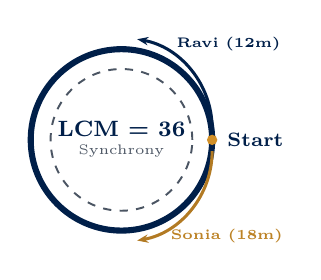
\begin{tikzpicture}[scale=0.72]
    % Circular track
    \draw[navy, line width=2.2pt] (0,0) circle (1.6cm);
    \draw[secondary, dashed, line width=0.7pt] (0,0) circle (1.25cm);
    \fill[gold] (1.6, 0) circle (2.6pt);
    \node[right=2pt, navy, font=\bfseries\scriptsize] at (1.6, 0) {Start};

    % Runners
    \draw[-{Stealth[length=4pt]}, primary, line width=1.1pt] (1.6, 0.2) arc (0:80:1.6cm);
    \node[above right, primary, font=\tiny\bfseries] at (0.8, 1.4) {Ravi (12m)};

    \draw[-{Stealth[length=4pt]}, gold!85!black, line width=1.1pt] (1.6, -0.2) arc (360:280:1.6cm);
    \node[below right, gold!90!black, font=\tiny\bfseries] at (0.7, -1.4) {Sonia (18m)};

    \node[navy, font=\bfseries\footnotesize] at (0, 0.2) {LCM = 36};
    \node[secondary, font=\tiny] at (0, -0.2) {Synchrony};
  \end{tikzpicture}
  \end{center}
\end{minipage}

\vspace{-0.5mm}
\subhead{Module 3 $\vert$ Worked Board Archetype 2: Maximum Sweet Stacking (HCF Model)}
\vspace{-1mm}

\begin{conceptBox}[title=Worked Model: Optimal Subdivision of Burfis,fonttitle=\bfseries\color{navy}]
  \textbf{Problem:} A sweet seller has $420$ kaju burfis and $130$ badam burfis. She wants to stack them such that each stack has the same number and they take up the least tray area. Find the maximum number of burfis per stack. \\
  \textbf{Solution:}\par
  \textbf{Step 1: Model.} Least tray area requires largest equal stacks leaving no remainder $\implies$ \textbf{Highest Common Factor} $\text{HCF}(420, 130)$. \\
  \textbf{Step 2: Prime factorizations.} $420 = 2^2 \times 3 \times 5 \times 7, \quad 130 = 2 \times 5 \times 13$. \\
  \textbf{Step 3: Compute HCF.} $\text{HCF}(420, 130) = 2^{\min(2, 1)} \times 5^{\min(1, 1)} = 2^1 \times 5^1 = \mathbf{10\text{ burfis per stack}}$. \\
  \textbf{Conclusion:} Each stack contains \textbf{10 burfis}. (Total stacks formed: $\frac{420}{10} + \frac{130}{10} = 42 + 13 = \mathbf{55\text{ stacks}}$).
\end{conceptBox}

\newpage

% =============================================================================
% PAGE 6: TERMINAL ZEROES & COMPOSITE NUMBER VERIFICATION
% =============================================================================
\thispagestyle{fancy}
\vspace*{0mm}

\chapterbanner{1}{TERMINAL ZEROES \& COMPOSITES}{The $2 \times 5$ Divisibility Lock \& Factoring Verifications}{\CoreTag}

\subhead{Module 1 $\vert$ Terminal Zeroes Analysis ($n$-th Powers)}

A perennial CBSE board exam question tests whether powers of an integer can terminate in the digit 0:

\begin{conceptBox}[title=The Fundamental Divisibility Lock for Terminal Zero,fonttitle=\bfseries\color{navy}]
  \textbf{Theorem:} A natural number ends with the digit 0 (i.e. has a terminal zero) if and only if it is a multiple of $10$. \\
  Since the prime factorization of $10$ is $2 \times 5$, any number ending in 0 \textbf{MUST contain BOTH 2 and 5} as prime factors in its prime decomposition.
\end{conceptBox}

\begin{minipage}[t]{0.58\textwidth}
  \subhead{Worked Board Archetype: Check if $6^n$ Ends in 0}
  \textbf{Question:} Check whether $6^n$ can end with the digit $0$ for any natural number $n \in \mathbb{N}$. \\
  \textbf{Rigorous Board Proof:}\par
  \textbf{Step 1: Factor the base.}
  $$6^n = (2 \times 3)^n = 2^n \times 3^n$$
  \textbf{Step 2: Apply the Uniqueness Clause of FTA.}
  The prime factors of $6^n$ are only $2$ and $3$. By the Fundamental Theorem of Arithmetic, this prime factorization is \textbf{unique}. There are no other primes in the factorization of $6^n$. \\
  \textbf{Step 3: State the contradiction and conclusion.}
  For $6^n$ to end with digit $0$, it must have $5$ as a prime factor. Since $5$ is absent from the prime factorization of $6^n$, \textbf{$6^n$ cannot end with the digit $0$ for any $n \in \mathbb{N}$}. $\blacksquare$
\end{minipage}\hfill
\begin{minipage}[t]{0.40\textwidth}
  \begin{center}
  \vspace{1mm}
  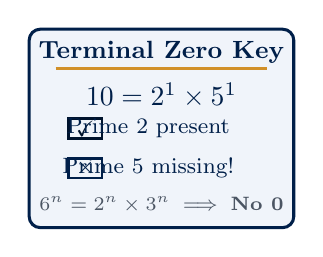
\begin{tikzpicture}[scale=0.84]
    % Lock & Key Engine
    \fill[bluepale, rounded corners=4pt] (-2,-1.4) rectangle (2,1.6);
    \draw[navy, line width=1.1pt, rounded corners=4pt] (-2,-1.4) rectangle (2,1.6);

    \node[navy, font=\bfseries\small] at (0, 1.25) {Terminal Zero Key};
    \draw[gold, line width=1pt] (-1.6, 1.0) -- (1.6, 1.0);

    % 10 = 2 x 5
    \node[navy, font=\bfseries\normalsize] at (0, 0.6) {$10 = 2^1 \times 5^1$};

    % Checkboxes
    \draw[green!60!black, line width=1pt] (-1.4, -0.05) rectangle (-0.9, 0.25);
    \node[green!60!black, font=\bfseries\footnotesize] at (-1.15, 0.1) {\checkmark};
    \node[navy, font=\footnotesize] at (-0.2, 0.1) {Prime $2$ present};

    \draw[reddeep, line width=1pt] (-1.4, -0.65) rectangle (-0.9, -0.35);
    \node[reddeep, font=\bfseries\footnotesize] at (-1.15, -0.5) {$\times$};
    \node[navy, font=\footnotesize] at (-0.2, -0.5) {Prime $5$ missing!};

    \node[secondary, font=\scriptsize\bfseries] at (0, -1.05) {$6^n = 2^n \times 3^n \implies \text{No 0}$};
  \end{tikzpicture}
  \end{center}
\end{minipage}

\vspace{1mm}
\subhead{Module 2 $\vert$ Algebraic Verification of Composite Numbers}

\begin{conceptBox}[title=Definition and Verification Protocol for Composite Numbers,fonttitle=\bfseries\color{navy}]
  \textbf{Definition:} A number is composite if it has \textbf{more than two factors} (i.e. factors other than 1 and itself). \\
  \textbf{Board Strategy:} NEVER expand the full arithmetic product! Instead, factor out the common term to prove that the expression is a product of two or more integers greater than 1.
\end{conceptBox}

\begin{minipage}[t]{0.485\textwidth}
  \begin{formulaBox}[title=Archetype 1: Expression with Addend 13,fonttitle=\bfseries\color{navy}]
    \textbf{Problem:} Explain why $7 \times 11 \times 13 + 13$ is a composite number. \\
    \textbf{Solution:}\par
    Take common factor $13$ outside:
    \begin{align*}
      7 \times 11 \times 13 + 13 &= 13 \times (7 \times 11 + 1) \\
      &= 13 \times (77 + 1) \\
      &= 13 \times 78 \\
      &= 13 \times (2 \times 3 \times 13) \\
      &= 2 \times 3 \times 13^2
    \end{align*}
    Since the given expression can be expressed as a product of prime factors $2, 3, 13$, it has factors other than 1 and itself. Hence, it is a \textbf{composite number}. $\blacksquare$
  \end{formulaBox}
\end{minipage}\hfill
\begin{minipage}[t]{0.485\textwidth}
  \begin{formulaBox}[title=Archetype 2: Factorial Expression + 5,fonttitle=\bfseries\color{navy}]
    \textbf{Problem:} Explain why $7 \times 6 \times 5 \times 4 \times 3 \times 2 \times 1 + 5$ is composite. \\
    \textbf{Solution:}\par
    Take common factor $5$ outside:
    \begin{align*}
      E &= 5 \times (7 \times 6 \times 4 \times 3 \times 2 \times 1 + 1) \\
      &= 5 \times (1008 + 1) \\
      &= 5 \times 1009
    \end{align*}
    Since $5$ and $1009$ are both integers greater than $1$, the number $E$ has at least $1, 5, 1009$, and $E$ as distinct positive factors. \\
    By definition of composite numbers, having more than two factors proves that $E$ is a \textbf{composite number}. $\blacksquare$
  \end{formulaBox}
\end{minipage}

\newpage

% =============================================================================
% PAGE 7: THE FUNDAMENTAL DIVISIBILITY LEMMA
% =============================================================================
\thispagestyle{fancy}
\vspace*{0mm}

\chapterbanner{1}{THE DIVISIBILITY LEMMA}{Theorem: If Prime $p$ Divides $a^2$, Then $p$ Divides $a$}{\CoreTag}

\subhead{Module 1 $\vert$ Theorem Statement \& Critical Mathematical Role}

\begin{conceptBox}[title=The Pillar of All Irrationality Proofs (Theorem 1.2),fonttitle=\bfseries\color{navy}]
  \textbf{Theorem:} \textit{Let $p$ be a prime number. If $p$ divides $a^2$ (where $a$ is a positive integer), then $p$ divides $a$.}
  $$\mathbf{p \mid a^2 \implies p \mid a \qquad (p \text{ is prime}, \, a \in \mathbb{Z}^+)}$$
  \textbf{Crucial Pedagogical Role:} This single lemma is the deductive engine of every square root irrationality proof in the CBSE curriculum. Without it, the contradiction cannot be established!
\end{conceptBox}

\vspace{0.4mm}
\begin{minipage}[t]{0.56\textwidth}
  \subhead{Module 2 $\vert$ Complete Formal Proof via FTA}
  \textbf{Proof:}\par
  \textbf{Step 1: Declare prime decomposition of $a$.} \\
  Let the prime factorization of $a$ be:
  $$a = p_1 p_2 p_3 \cdots p_n$$
  where $p_1, p_2, \dots, p_n$ are primes (not necessarily distinct). \\
  \textbf{Step 2: Square both sides.}
  $$a^2 = (p_1 p_2 \cdots p_n)(p_1 p_2 \cdots p_n) = p_1^2 p_2^2 \cdots p_n^2$$
  \textbf{Step 3: Apply the divisibility condition.} \\
  We are given that prime $p$ divides $a^2$ ($p \mid a^2$). \\
  \textbf{Step 4: Invoke the Uniqueness of FTA.} \\
  By the Fundamental Theorem of Arithmetic, the prime factorization of $a^2$ is \textbf{unique}. The only prime factors of $a^2$ are $p_1, p_2, \dots, p_n$. \\
  Therefore, $p$ must be one of the prime factors $p_1, p_2, \dots, p_n$. \\
  \textbf{Step 5: Conclude divisibility of $a$.} \\
  Since $a = p_1 p_2 \cdots p_n$ and $p \in \{p_1, p_2, \dots, p_n\}$, it follows directly that \textbf{$p$ divides $a$}. $\blacksquare$
\end{minipage}\hfill
\begin{minipage}[t]{0.42\textwidth}
  \begin{center}
  \vspace{1mm}
  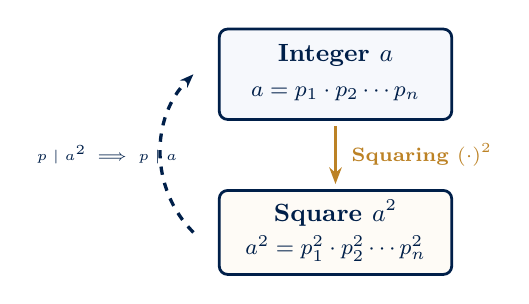
\begin{tikzpicture}[scale=0.82]
    % Squaring Mapping
    \draw[navy, line width=1pt, fill=bluepale!60, rounded corners=3pt] (-1.8, 1.8) rectangle (1.8, 3.2);
    \node[navy, font=\bfseries\small] at (0, 2.8) {Integer $a$};
    \node[navy, font=\footnotesize] at (0, 2.2) {$a = p_1 \cdot p_2 \cdots p_n$};

    \draw[-{Stealth[length=6pt]}, gold!90!black, line width=1.4pt] (0, 1.7) -- (0, 0.8);
    \node[right, gold!90!black, font=\bfseries\scriptsize] at (0.1, 1.25) {Squaring $(\cdot)^2$};

    \draw[navy, line width=1pt, fill=goldpale!70, rounded corners=3pt] (-1.8, -0.6) rectangle (1.8, 0.7);
    \node[navy, font=\bfseries\small] at (0, 0.35) {Square $a^2$};
    \node[navy, font=\footnotesize] at (0, -0.2) {$a^2 = p_1^2 \cdot p_2^2 \cdots p_n^2$};

    % Divisibility pointer
    \draw[-{Stealth[length=5pt]}, primary, dashed, line width=1.2pt] (-2.2, 0.05) to[bend left=45] (-2.2, 2.5);
    \node[left, primary, font=\bfseries\tiny] at (-2.3, 1.25) {$p \mid a^2 \implies p \mid a$};
  \end{tikzpicture}
  \end{center}
\end{minipage}

\vspace{0.8mm}
\subhead{Module 3 $\vert$ Why Primality of $p$ is Strictly Necessary (Counterexamples)}

\begin{warningBox}[title=Fatal Error: The Lemma FAILS if $p$ is a Composite Number!,fonttitle=\bfseries\color{navy}]
  \textbf{Crucial Distinction:} The theorem holds \textbf{ONLY} when $p$ is prime. If $p$ is composite, the implication $p \mid a^2 \implies p \mid a$ is \textbf{FALSE}! \\
  \textbf{Counterexample 1:} Let $p = 4$ (composite) and $a = 6$.
  \begin{itemize}[itemsep=0pt]
    \item $a^2 = 6^2 = 36$. Here $4$ divides $36$ ($36 = 4 \times 9$).
    \item But $4$ does \textbf{NOT} divide $6$ ($6/4 = 1.5 \notin \mathbb{Z}$)!
  \end{itemize}
  \textbf{Why does this happen?} A composite number can split its prime factors across the two copies of $a$: $4 = 2 \times 2$, where one $2$ divides the first $a$ and the other $2$ divides the second $a$. A prime number is indivisible and cannot split; it must belong entirely to $a$ itself!
\end{warningBox}

\newpage

% =============================================================================
% PAGE 8: PROOFS OF IRRATIONALITY: PURE SURDS
% =============================================================================
\thispagestyle{fancy}
\vspace*{0mm}

\chapterbanner{1}{PROOFS OF IRRATIONALITY: PURE SURDS}{The Contradiction Method \& Rigorous Board Template for $\sqrt{5}$}{\WorkedTag}

\subhead{Module 1 $\vert$ The Reductio ad Absurdum (Proof by Contradiction) Architecture}

\begin{conceptBox}[title=Four-Step Universal Contradiction Template,fonttitle=\bfseries\color{navy}]
  \begin{enumerate}[leftmargin=5mm,itemsep=1pt]
    \item \textbf{Negation Assumption:} Assume the contrary: that $\sqrt{p}$ is rational ($\sqrt{p} = \frac{a}{b}$, with $a, b \in \mathbb{Z}^+, \gcd(a, b) = 1$).
    \item \textbf{First Divisibility Deduction:} Square both sides to establish $p b^2 = a^2 \implies p \mid a^2 \implies \mathbf{p \mid a}$.
    \item \textbf{Second Divisibility Deduction:} Substitute $a = pc$ to establish $b^2 = p c^2 \implies p \mid b^2 \implies \mathbf{p \mid b}$.
    \item \textbf{Contradiction \& Verdict:} $a$ and $b$ share common factor $p$, contradicting $\gcd(a, b) = 1$. Hence, $\sqrt{p}$ is irrational.
  \end{enumerate}
\end{conceptBox}

\vspace{0.4mm}
\subhead{Module 2 $\vert$ Standard Board Exam Model Proof: $\sqrt{5}$ is Irrational}

\begin{formulaBox}[title=Complete Full-Mark CBSE Solution Protocol,fonttitle=\bfseries\color{navy}]
  \textbf{Theorem:} Prove that $\sqrt{5}$ is an irrational number. \\
  \textbf{Proof:}\par
  \textbf{Step 1: State the contradiction hypothesis.} \\
  Let us assume, to the contrary, that $\sqrt{5}$ is a rational number. \\
  Therefore, there exist positive integers $a$ and $b$ ($b \ne 0$) such that:
  $$\mathbf{\sqrt{5} = \frac{a}{b}}, \quad \text{where } a \text{ and } b \text{ are \textbf{coprime}} \ (\text{i.e. } \gcd(a, b) = 1).$$
  \textbf{Step 2: Square both sides and deduce divisibility of $a$.} \\
  Cross-multiplying: $b\sqrt{5} = a$. \\
  Squaring both sides:
  $$\mathbf{5b^2 = a^2} \qquad \text{--- (Equation 1)}$$
  Since $5$ divides $5b^2$, it follows that \textbf{$5$ divides $a^2$}. \\
  By Theorem (since $5$ is a prime number), \textbf{$5$ divides $a$}. \quad --- (Statement A) \\[2pt]
  \textbf{Step 3: Express $a$ and deduce divisibility of $b$.} \\
  Since $5$ divides $a$, we can write $\mathbf{a = 5c}$ for some integer $c$. \\
  Substituting $a = 5c$ into Equation (1):
  $$5b^2 = (5c)^2 = 25c^2 \implies \mathbf{b^2 = 5c^2} \qquad \text{--- (Equation 2)}$$
  Since $5$ divides $5c^2$, it follows that \textbf{$5$ divides $b^2$}. \\
  By Theorem (since $5$ is prime), \textbf{$5$ divides $b$}. \quad --- (Statement B) \\[2pt]
  \textbf{Step 4: Establish the mathematical contradiction.} \\
  From Statement A and Statement B, \textbf{$5$ is a common factor of both $a$ and $b$}. \\
  This contradicts our initial foundational assumption that $a$ and $b$ are coprime (having no common factor other than $1$). \\[2pt]
  \textbf{Step 5: Write the mandatory closing conclusion.} \\
  This contradiction has arisen because of our incorrect assumption that $\sqrt{5}$ is rational. \\
  Hence, we conclude that \textbf{$\sqrt{5}$ is an irrational number}. $\blacksquare$
\end{formulaBox}

\vspace{0.4mm}
\subhead{Module 3 $\vert$ Universal Transformation for $\sqrt{2}$ and $\sqrt{3}$}

To prove $\sqrt{2}$ or $\sqrt{3}$ is irrational, use the \textbf{identical template} with the exact numerical replacements:
$$\sqrt{2}: \quad 2b^2 = a^2 \implies 2 \mid a \implies a = 2c \implies b^2 = 2c^2 \implies 2 \mid b \implies \text{Contradiction with } \gcd(a, b)=1$$
$$\sqrt{3}: \quad 3b^2 = a^2 \implies 3 \mid a \implies a = 3c \implies b^2 = 3c^2 \implies 3 \mid b \implies \text{Contradiction with } \gcd(a, b)=1$$

\newpage

% =============================================================================
% PAGE 9: PROOFS OF IRRATIONALITY: LINEAR COMBINATIONS
% =============================================================================
\thispagestyle{fancy}
\vspace*{0mm}

\chapterbanner{1}{PROOFS OF IRRATIONALITY: COMBINATIONS}{Linear Sums, Differences, Products \& Quotients}{\WorkedTag}

\subhead{Module 1 $\vert$ The "Given $\sqrt{p}$ is Irrational" Board Protocol}

\begin{conceptBox}[title=Algebraic Rearrangement vs. Full Contradiction,fonttitle=\bfseries\color{navy}]
  \textbf{CBSE Marking Scheme Rule:} When an exam question states: \textit{"Given that $\sqrt{5}$ is irrational, prove that $3 + 2\sqrt{5}$ is irrational"}:
  \begin{itemize}[leftmargin=4mm]
    \item Do \textbf{NOT} reprove $\sqrt{5}$ from scratch!
    \item Simply isolate the irrational surd $\sqrt{5}$ on the LHS using basic algebra.
    \item Show that the RHS consists entirely of rational operations on integers, creating an immediate contradiction between $\mathbb{Q}'$ and $\mathbb{Q}$.
  \end{itemize}
\end{conceptBox}

\vspace{0.4mm}
\begin{minipage}[t]{0.56\textwidth}
  \subhead{Module 2 $\vert$ Worked Archetype: $3 + 2\sqrt{5}$}
  \textbf{Problem:} Given that $\sqrt{5}$ is irrational, prove that $3 + 2\sqrt{5}$ is irrational. \\
  \textbf{Solution:}\par
  \textbf{Step 1: Assumption.} \\
  Assume, to the contrary, that $3 + 2\sqrt{5}$ is rational. \\
  Let $3 + 2\sqrt{5} = \frac{a}{b}$, where $a, b \in \mathbb{Z}, b \ne 0, \gcd(a, b) = 1$. \\
  \textbf{Step 2: Isolate the surd $\sqrt{5}$.}
  $$2\sqrt{5} = \frac{a}{b} - 3 = \frac{a - 3b}{b} \implies \mathbf{\sqrt{5} = \frac{a - 3b}{2b}}$$
  \textbf{Step 3: Analyze rationality.} \\
  Since $a$ and $b$ are integers, $a - 3b$ and $2b$ are integers with $2b \ne 0$. Therefore, $\frac{a - 3b}{2b}$ is a rational number. \\
  This implies that $\sqrt{5}$ is rational. \\
  \textbf{Step 4: State contradiction and verdict.} \\
  But this contradicts the fact that $\sqrt{5}$ is irrational. \\
  Hence, our assumption is false. \textbf{$3 + 2\sqrt{5}$ is irrational}. $\blacksquare$
\end{minipage}\hfill
\begin{minipage}[t]{0.42\textwidth}
  \begin{center}
  \vspace{1mm}
  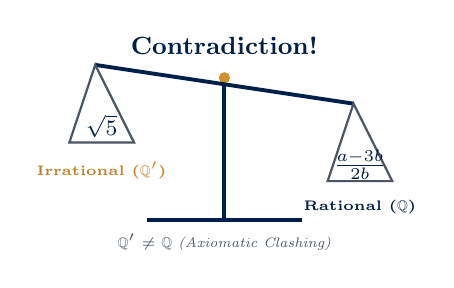
\begin{tikzpicture}[scale=0.82]
    % Balance scale visual
    \draw[navy, line width=1.5pt] (0, 0) -- (0, 2.2);
    \draw[navy, line width=1.2pt] (-1.2, 0) -- (1.2, 0); % base
    \fill[gold] (0, 2.2) circle (2.5pt);

    % Crossbeam tilted
    \draw[navy, line width=1.4pt] (-2.0, 2.4) -- (2.0, 1.8);

    % Left pan: Surd
    \draw[secondary, line width=0.8pt] (-2.0, 2.4) -- (-2.4, 1.2) -- (-1.4, 1.2) -- cycle;
    \node[primary, font=\bfseries\footnotesize] at (-1.9, 1.45) {$\sqrt{5}$};
    \node[below, gold!90!black, font=\bfseries\tiny] at (-1.9, 1.05) {Irrational ($\mathbb{Q}'$)};

    % Right pan: Rational expression
    \draw[secondary, line width=0.8pt] (2.0, 1.8) -- (1.6, 0.6) -- (2.6, 0.6) -- cycle;
    \node[primary, font=\bfseries\footnotesize] at (2.1, 0.85) {$\frac{a-3b}{2b}$};
    \node[below, navy, font=\bfseries\tiny] at (2.1, 0.45) {Rational ($\mathbb{Q}$)};

    \node[navy, font=\bfseries\small] at (0, 2.7) {Contradiction!};
    \node[secondary, font=\tiny\itshape] at (0, -0.35) {$\mathbb{Q}' \ne \mathbb{Q}$ (Axiomatic Clashing)};
  \end{tikzpicture}
  \end{center}
\end{minipage}

\vspace{0.8mm}
\subhead{Module 3 $\vert$ Worked Archetypes: Difference \& Quotient Forms}

\begin{minipage}[t]{0.485\textwidth}
  \begin{formulaBox}[title=Archetype: Difference Form ($5 - \sqrt{3}$),fonttitle=\bfseries\color{navy}]
    \textbf{Problem:} Prove that $5 - \sqrt{3}$ is irrational. \\
    \textbf{Solution:}\par
    Let $5 - \sqrt{3} = \frac{a}{b}$ ($a, b \in \mathbb{Z}, b \ne 0$). \\
    Rearrange to isolate $\sqrt{3}$:
    $$\sqrt{3} = 5 - \frac{a}{b} = \frac{5b - a}{b}$$
    Since $a, b$ are integers, $\frac{5b - a}{b}$ is rational. \\
    This implies $\sqrt{3}$ is rational, contradicting the known fact that $\sqrt{3}$ is irrational. \\
    $\therefore \mathbf{5 - \sqrt{3}}$ is an \textbf{irrational number}. $\blacksquare$
  \end{formulaBox}
\end{minipage}\hfill
\begin{minipage}[t]{0.485\textwidth}
  \begin{formulaBox}[title=Archetype: Quotient Form ($1/\sqrt{2}$),fonttitle=\bfseries\color{navy}]
    \textbf{Problem:} Prove that $\frac{1}{\sqrt{2}}$ is irrational. \\
    \textbf{Solution:}\par
    Let $\frac{1}{\sqrt{2}} = \frac{a}{b}$ ($a, b \in \mathbb{Z}, a \ne 0, b \ne 0$). \\
    Inverting both sides:
    $$\sqrt{2} = \frac{b}{a}$$
    Since $a, b \in \mathbb{Z}$ and $a \ne 0$, $\frac{b}{a}$ is rational. \\
    This implies $\sqrt{2}$ is rational, which contradicts the fact that $\sqrt{2}$ is irrational. \\
    $\therefore \mathbf{\frac{1}{\sqrt{2}}}$ is an \textbf{irrational number}. $\blacksquare$
  \end{formulaBox}
\end{minipage}

\newpage

% =============================================================================
% PAGE 10: MASTER CONCEPT & FORMULA REVISION MATRIX
% =============================================================================
\thispagestyle{fancy}
\vspace*{0mm}

\chapterbanner{1}{QUICK-REVISION MATRIX}{Comprehensive Formula Table, Decision Rules \& Board Conventions}{\ReferenceTag}

\subhead{Module 1 $\vert$ Master Formula \& Conceptual Rules Matrix}

\begin{center}
{\small
\begin{tabularx}{\textwidth}{@{}lXXl@{}}
  \toprule
  \textbf{\color{navy}Concept / Theorem} & \textbf{\color{navy}Mathematical Formula} & \textbf{\color{navy}Key Domain Restriction} & \textbf{\color{navy}CBSE Exam Utility} \\
  \midrule
  \textbf{FTA Decomposition} & $n = \prod_{i=1}^k p_i^{a_i}$ & $p_1 < p_2 < \dots < p_k$ primes, $a_i \ge 1$ & Canonical representation. \\
  \addlinespace[1.5pt]
  \textbf{HCF by Primes} & $\text{HCF}(a, b) = \prod p_i^{\min(\alpha_i, \beta_i)}$ & Common prime factors only & Subdividing, equal stacks. \\
  \addlinespace[1.5pt]
  \textbf{LCM by Primes} & $\text{LCM}(a, b) = \prod p_i^{\max(\alpha_i, \beta_i)}$ & All prime factors involved & Cycles, bells, laps. \\
  \addlinespace[1.5pt]
  \textbf{Two-Number Law} & $\text{HCF}(a, b) \times \text{LCM}(a, b) = a \cdot b$ & \textbf{Valid ONLY for 2 numbers} & Missing quantity calculation. \\
  \addlinespace[1.5pt]
  \textbf{Three-Number Rule} & $\text{HCF} \times \text{LCM} \ne a \cdot b \cdot c$ & Product law strictly fails & Always use prime powers. \\
  \addlinespace[1.5pt]
  \textbf{Terminal Zeroes} & $N = 2^n \times 5^m \times k$ ($n, m \ge 1$) & Requires BOTH $2$ and $5$ primes & $4^n, 6^n, 12^n$ cannot end in $0$. \\
  \addlinespace[1.5pt]
  \textbf{Composite Proof} & $N = k \times m$ ($k, m > 1$) & Has $>2$ distinct positive factors & Factor out common addend. \\
  \addlinespace[1.5pt]
  \textbf{Divisibility Lemma} & $p \mid a^2 \implies p \mid a$ & \textbf{$p$ MUST be prime} & Foundation of surd proofs. \\
  \addlinespace[1.5pt]
  \textbf{Pure Surd Proof} & $\sqrt{p} = a/b \implies p b^2 = a^2$ & $a, b$ coprime integers ($\gcd=1$) & Contradiction template. \\
  \addlinespace[1.5pt]
  \textbf{Linear Combo Proof} & $\sqrt{p} = \frac{a - r b}{s b}$ & Isolate surd on LHS & LHS $\in \mathbb{Q}'$, RHS $\in \mathbb{Q}$ clash. \\
  \bottomrule
\end{tabularx}}
\end{center}

\vspace{0.5mm}
\subhead{Module 2 $\vert$ Board Question Diagnostic Flowchart}

\begin{center}
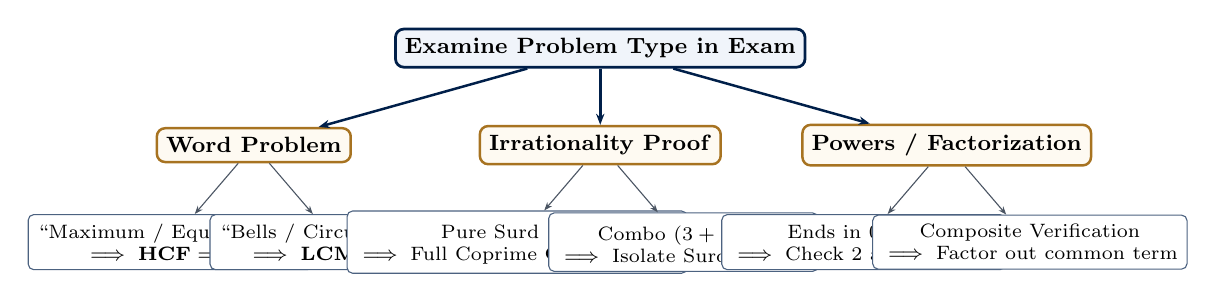
\begin{tikzpicture}[scale=0.88, every node/.style={font=\footnotesize}]
  % Decision Tree
  \node[draw=navy, fill=bluepale, rounded corners=3pt, line width=1pt] (Q) at (0, 3.2) {\textbf{Examine Problem Type in Exam}};

  \node[draw=gold!80!black, fill=goldpale, rounded corners=3pt, line width=0.9pt] (W) at (-5.0, 1.8) {\textbf{Word Problem}};
  \node[draw=gold!80!black, fill=goldpale, rounded corners=3pt, line width=0.9pt] (I) at (0, 1.8) {\textbf{Irrationality Proof}};
  \node[draw=gold!80!black, fill=goldpale, rounded corners=3pt, line width=0.9pt] (P) at (5.0, 1.8) {\textbf{Powers / Factorization}};

  \draw[-{Stealth[length=4pt]}, navy, line width=0.9pt] (Q) -- (W);
  \draw[-{Stealth[length=4pt]}, navy, line width=0.9pt] (Q) -- (I);
  \draw[-{Stealth[length=4pt]}, navy, line width=0.9pt] (Q) -- (P);

  % Leaves for Word Problem
  \node[draw=navy!70, fill=white, rounded corners=2pt, font=\scriptsize, align=center] (WH) at (-6.2, 0.4) {``Maximum / Equal stacks''\\$\implies \mathbf{HCF = \min}$};
  \node[draw=navy!70, fill=white, rounded corners=2pt, font=\scriptsize, align=center] (WL) at (-3.8, 0.4) {``Bells / Circular Track''\\$\implies \mathbf{LCM = \max}$};
  \draw[-{Stealth[length=3pt]}, secondary] (W) -- (WH);
  \draw[-{Stealth[length=3pt]}, secondary] (W) -- (WL);

  % Leaves for Irrationality
  \node[draw=navy!70, fill=white, rounded corners=2pt, font=\scriptsize, align=center] (IP) at (-1.2, 0.4) {Pure Surd ($\sqrt{5}$)\\$\implies \text{Full Coprime Contradiction}$};
  \node[draw=navy!70, fill=white, rounded corners=2pt, font=\scriptsize, align=center] (IC) at (1.2, 0.4) {Combo ($3+2\sqrt{5}$)\\$\implies \text{Isolate Surd on LHS}$};
  \draw[-{Stealth[length=3pt]}, secondary] (I) -- (IP);
  \draw[-{Stealth[length=3pt]}, secondary] (I) -- (IC);

  % Leaves for Powers
  \node[draw=navy!70, fill=white, rounded corners=2pt, font=\scriptsize, align=center] (PT) at (3.8, 0.4) {Ends in $0$ ($6^n$)?\\$\implies \text{Check } 2 \text{ and } 5 \text{ factors}$};
  \node[draw=navy!70, fill=white, rounded corners=2pt, font=\scriptsize, align=center] (PC) at (6.2, 0.4) {Composite Verification\\$\implies \text{Factor out common term}$};
  \draw[-{Stealth[length=3pt]}, secondary] (P) -- (PT);
  \draw[-{Stealth[length=3pt]}, secondary] (P) -- (PC);
\end{tikzpicture}
\end{center}

\vspace{0.5mm}
\subhead{Module 3 $\vert$ Curriculum Scope Verification (CBSE 2026--27)}

\begin{center}
{\footnotesize
\begin{tabularx}{\textwidth}{@{}lXl@{}}
  \toprule
  \textbf{\color{navy}Syllabus Status} & \textbf{\color{navy}Curriculum Topic} & \textbf{\color{navy}Action Plan for CBSE Exam} \\
  \midrule
  \textbf{\color{green!60!black}Active Scope} & Fundamental Theorem of Arithmetic (FTA) \& Canonical Decomposition & Master prime power factorization and factor trees. \\
  \textbf{\color{green!60!black}Active Scope} & Proofs of Irrationality of $\sqrt{2}, \sqrt{3}, \sqrt{5}$ and linear combinations & Write all 5 steps with explicit "coprime" statement. \\
  \textbf{\color{reddeep}DELETED} & Euclid's Division Lemma ($a = bq + r$) \& Long Division HCF & \textbf{Do NOT study} (Zero marks allotted). \\
  \textbf{\color{reddeep}DELETED} & Decimal Expansions of Rationals ($q = 2^n 5^m$ terminating checks) & \textbf{Do NOT study} (Completely deleted from syllabus). \\
  \bottomrule
\end{tabularx}}
\end{center}

\newpage

% =============================================================================
% PAGE 11: CBSE BOARD EXAM TRAPS, ARITHMETIC HACKS & AUDIT CHECKLIST
% =============================================================================
\thispagestyle{fancy}
\vspace*{0mm}

\chapterbanner{1}{BOARD STRATEGY \& AUDIT}{The 5 Fatal Examiner Traps, Arithmetic Hacks \& Audit Protocol}{\ExamTag}

\subhead{Module 1 $\vert$ The Five Lethal CBSE Board Exam Traps}

\begin{warningBox}[title=Examiner Trap Alerts (Where Students Lose Marks),fonttitle=\bfseries\color{navy}]
  \begin{enumerate}[leftmargin=4mm,itemsep=1pt,topsep=1pt]
    \item \textbf{Trap 1: Omitting "Coprime" in Proof by Contradiction (-1 Mark).} Writing $\sqrt{5} = a/b$ without explicitly stating \textit{"$a, b$ are coprime integers ($b \ne 0$)"} destroys the contradiction premise.
    \item \textbf{Trap 2: Applying Two-Number Product Law to Three Numbers.} Writing $\text{HCF}(a, b, c) \times \text{LCM}(a, b, c) = a \cdot b \cdot c$ is false! For 3 numbers, always use prime factorization directly.
    \item \textbf{Trap 3: Multiplying Out in Composite Proofs.} In \textit{"Explain why $7 \times 11 \times 13 + 13$ is composite"}, do NOT multiply to $1014$. \textbf{Always factor out common addend:} $13(7 \times 11 + 1) = 13 \times 78$.
    \item \textbf{Trap 4: Confusing HCF and LCM in Context.} If the answer must be smaller than the given numbers (e.g. stack size, container capacity), it is \textbf{HCF}. If larger (e.g. time until next bell, laps), it is \textbf{LCM}.
    \item \textbf{Trap 5: Incomplete Closing Contradiction Statement.} Ending abruptly after $5 \mid b$ without stating \textit{"This contradicts coprimality of $a, b$, which arose from our incorrect assumption..."} loses marks.
  \end{enumerate}
\end{warningBox}

\vspace{-1mm}
\subhead{Module 2 $\vert$ Rapid Arithmetic Verification Hacks}
\vspace{-1mm}

\begin{minipage}[t]{0.60\textwidth}
  \begin{conceptBox}[title=Sanity Checks for Real Numbers,fonttitle=\bfseries\color{navy}]
    \begin{itemize}[leftmargin=4mm,itemsep=1pt,topsep=1pt]
      \item \textbf{Divisibility Invariance:} $\text{LCM}(a, b)$ must be \textbf{strictly divisible} by $\text{HCF}(a, b)$. If $\text{LCM} \pmod{\text{HCF}} \ne 0$, your calculation has an arithmetic error!
      \item \textbf{Size Bounds:} $\text{HCF}(a, b) \le \min(a, b) \le \max(a, b) \le \text{LCM}(a, b)$.
      \item \textbf{Coprime Rule:} If $\text{HCF}(a, b) = 1$, then $\text{LCM}(a, b) = a \times b$.
    \end{itemize}
  \end{conceptBox}
\end{minipage}\hfill
\begin{minipage}[t]{0.38\textwidth}
  \begin{center}
  
\begin{tikzpicture}[scale=0.68]
    % Audit Shield Emblem
    \draw[navy, line width=1.4pt, fill=bluepale!60] 
      (0, 1.6) -- (1.3, 1.15) -- (1.3, -0.2) to[out=270, in=0] (0, -1.6) to[out=180, in=270] (-1.3, -0.2) -- (-1.3, 1.15) -- cycle;
    \draw[gold, line width=0.9pt] 
      (0, 1.45) -- (1.15, 1.05) -- (1.15, -0.15) to[out=270, in=0] (0, -1.4) to[out=180, in=270] (-1.15, -0.15) -- (-1.15, 1.05) -- cycle;

    \node[navy, font=\bfseries\normalsize] at (0, 0.6) {MM};
    \node[gold!90!black, font=\bfseries\tiny] at (0, 0.15) {100\% AUDIT};
    \node[navy, font=\bfseries\tiny] at (0, -0.3) {CBSE 2026--27};
    \node[secondary, font=\tiny\itshape] at (0, -0.75) {Zero Marks Lost};
  \end{tikzpicture}
  \end{center}
\end{minipage}

\vspace{-1mm}
\subhead{Module 3 $\vert$ The Maths Manthan 5-Point Pre-Submission Audit Protocol}
\vspace{-1mm}

\begin{successBox}[title=Pre-Submission Verification Checklist,fonttitle=\bfseries\color{navy}]
  {\footnotesize
  \begin{tabularx}{\textwidth}{@{}clX@{}}
    \toprule
    \textbf{Check} & \textbf{Audit Stage} & \textbf{Verification Action Before Handing in Your Answer Sheet} \\
    \midrule
    $\square$ & \textbf{1. Coprime Clause} & In every irrationality proof, did I write $\gcd(a, b) = 1$ with $a, b \in \mathbb{Z}^+$ and $b \ne 0$? \\
    \addlinespace[1pt]
    $\square$ & \textbf{2. Theorem Attribution} & Did I explicitly quote \textit{"By the Fundamental Theorem of Arithmetic"} or \textit{"Since $p$ is prime"}? \\
    \addlinespace[1pt]
    $\square$ & \textbf{3. Product Theorem Audit} & If calculating for two numbers, did I verify that $\text{HCF} \times \text{LCM}$ equals $a \times b$? \\
    \addlinespace[1pt]
    $\square$ & \textbf{4. Terminal Zero Logic} & Did I explicitly show that the prime decomposition lacks the factor $5$ (or $2$)? \\
    \addlinespace[1pt]
    $\square$ & \textbf{5. Unit \& Wording Check} & In word problems, did I include physical units (minutes, sweets, meters) in the final sentence? \\
    \bottomrule
  \end{tabularx}}
\end{successBox}

\vspace{1mm}
\begin{center}
  {\footnotesize\bfseries\color{navy}End of Chapter 1 Master Handbook \quad$\vert$\quad Maths Manthan Tuition Classes}\\[0.5mm]
  {\scriptsize\color{muted}Helpline: +91-8171546558 \quad$\vert$\quad contact@mathsmanthan.co.in \quad$\vert$\quad https://mathsmanthan.co.in}
\end{center}

\end{document}
